\documentclass[12pt,a4paper]{article}
\usepackage[polish]{babel}
\usepackage[utf8]{inputenc}
\usepackage[T1]{fontenc}
\usepackage{pslatex} %z tym czcionka wygląda ładniej

\usepackage{xcolor}
\definecolor{CodeListingColor}{rgb}{0.95,0.95,0.95}
\usepackage{minted}

\usepackage{mathtools}
\DeclarePairedDelimiter\ceil{\lceil}{\rceil}
\DeclarePairedDelimiter\floor{\lfloor}{\rfloor}


\setlength\parindent{0pt} %żeby wcięć przed akapitem nie było

%\author{
%  Ewa Fengler 132219
%  \and
%  Dariusz Grynia 132235
%  \and
%  gr. I1, wt. godz. 15.10, tyg. parzyste
%}
\date{}
\title{Przetwarzanie równoległe - \\ Projekt 1 OMP}

\usepackage[a4paper, left=2.5cm, right=2.5cm, top=2.5cm, bottom=2.5cm, headsep=1.2cm]{geometry}
\usepackage[figurename=Rys.]{caption}
\usepackage{graphicx}
\usepackage[space]{grffile}
\usepackage{float}
%\usepackage{etoolbox}
%\makeatletter
%\patchcmd{\Ginclude@eps}{"#1"}{#1}{}{}
%\makeatother

\begin{document}
\maketitle
\thispagestyle{empty}

\vspace{1cm}
\section{Wstęp}

Ewa Fengler 132219

Dariusz Grynia 132235

grupa I1,\\
wtorki godz. 15.10,\\
tygodnie parzyste\\
dariusz.grynia@student.put.poznan.pl\\


Mnożenie macierzy - porównanie efektywności metod –
\begin{itemize}

\item 3 pętle - kolejność pętli: ijk, podział pracy przed pętlą 1
\item 6 pętli - kolejność pętli: zewnętrznych ijk, wewnętrznych: ii,jj,kk podział pracy przed pętlą 1.
\end{itemize}


\section{Analiza z przygotowania eksperymentu}


\subsection{Kod}
\begin{listing}[H]
\begin{minted}
[
	frame=lines,
	framesep=2mm,
	baselinestretch=1.2,
	tabsize=2,
	bgcolor=CodeListingColor,
	%fontsize=\footnotesize,
	linenos %Enables line numbers
]{c++}
void multiply_matrices_IJK(){
#pragma omp parallel for
	for (int i = 0; i < SIZE; i++)
		for (int j = 0; j < SIZE; j++)
			for (int k = 0; k < SIZE; k++)
				matrix_r[i][j] += matrix_a[i][k] * matrix_b[k][j];
}
\end{minted}
\caption{Kod metody 3 pętlowej, kolejność pętli IJK, podział pracy przed pierwszą pętlą}
\label{lst:ijk}
\end{listing}

\begin{listing}[H]
\begin{minted}
[
	frame=lines,
	framesep=2mm, %frame separation
	baselinestretch=1.2, %Interlining of the code
	obeytabs=true,
	tabsize=2, %number of spaces a tab is equivalent to
	bgcolor=CodeListingColor,
	%fontsize=\footnotesize,
	linenos %Enables line numbers
]{c++}

void multiply_matrices_IJK_IJK(){
#pragma omp parallel for
	for (int i = 0; i < SIZE; i += R)
		for (int j = 0; j < SIZE; j += R)
			for (int k = 0; k < SIZE; k += R)
				for (int ii = i; ii < i + R; ii++)
					for (int jj = j; jj < j + R; jj++)
						for (int kk = k; kk < k + R; kk++)
							matrix_r[ii][jj] += matrix_a[ii][kk] * matrix_b[kk][jj];
}

\end{minted}
\caption{Kod metody 6 pętlowej, kolejność pętli IJK-IJK, podział pracy przed pierwszą pętlą}
\label{lst:ijkiijjkk}
\end{listing}

\subsection{Wyścig}

\subsection{Analiza podziału pracy na wątki}


\subsubsection{Metoda 3 pętlowa, kolejność pętli IJK, podział pracy przed pierwszą pętlą}

\begin{figure}[H]
  \centering
    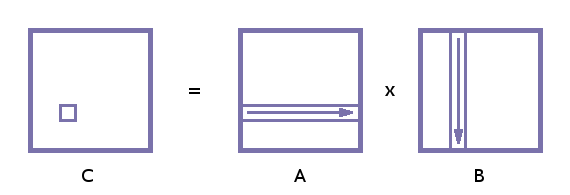
\includegraphics[width=0.60\textwidth]{IJK_K.jpg}
    \caption{obszar danych wykorzystywanych w wewnętrznej pętli}
\end{figure}

W jednej iteracji pętli wewnętrznej pojedynczy wątek przechodzi raz wiersz macierzy A, raz kolumnę macierzy B i zapisuje wartość do jednego pola macierzy wynikowej C.

\begin{figure}[H]
  \centering
    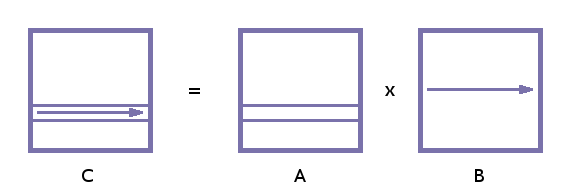
\includegraphics[width=0.60\textwidth]{IJK_KJ.jpg}
    \caption{obszar danych wykorzystywanych w dwóch wewnętrznych pętlach}
\end{figure}

Wykonując dwie pętle wewnętrzne, pojedynczy wątek przechodzi wielokrotnie wiersz macierzy A, przechodzi raz każdą kolumnę macierzy B i przechodzi wiersz macierzy C jeden raz.

\begin{figure}[H]
  \centering
    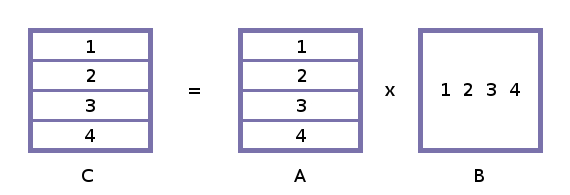
\includegraphics[width=0.60\textwidth]{IJK_KJI.jpg}
    \caption{podział pracy na wątki}
\end{figure}

podział pracy następuje przed najbardziej zewnętrzną pętlą. Każdy wątek przechodzi osobne wiersze macierzy A i C oraz całą macierz B.

\subsubsection{Metoda 6 pętlowa, kolejność pętli IJK-IJK, podział pracy przed pierwszą pętlą}

\begin{figure}[H]
  \centering
    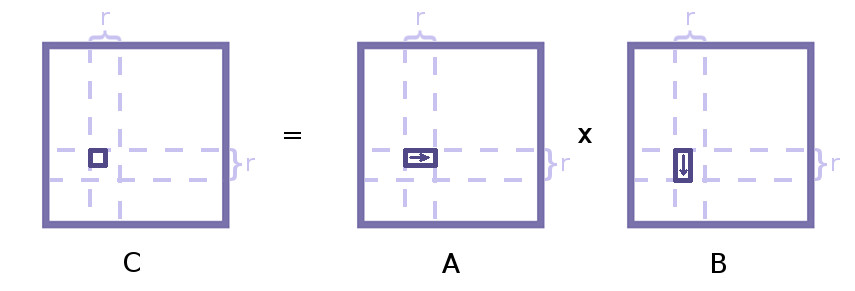
\includegraphics[width=0.60\textwidth]{IJKIJK_KK.jpg}
    \caption{obszar danych wykorzystywanych w wewnętrznej pętli}
\end{figure}

W jednej iteracji pętli wewnętrznej pojedynczy wątek przechodzi raz fragment wiersza długości r macierzy A, raz fragment kolumny długości r macierzy B i zapisuje wartość do jednego pola macierzy C.

\begin{figure}[H]
  \centering
    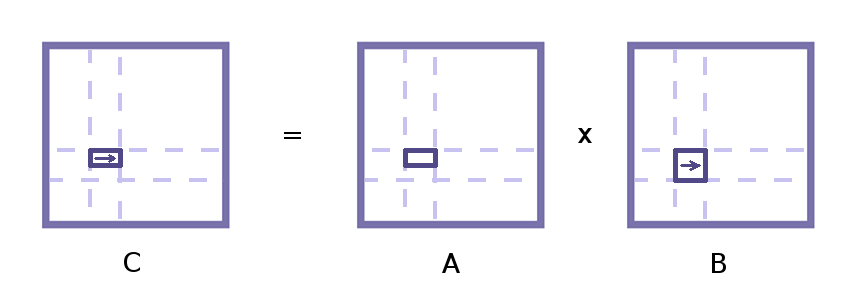
\includegraphics[width=0.60\textwidth]{IJKIJK_KKJJ.jpg}
    \caption{obszar danych wykorzystywanych w dwóch wewnętrznych pętlach}
\end{figure}

Wykonując dwie pętle wewnętrzne, pojedynczy wątek przechodzi wielokrotnie fragment wiersza długości r macierzy A, przechodzi raz każdą kolumnę fragmentu macierzy B o rozmiarze r x r i przechodzi jednokrotnie fragment wiersza długości r macierzy wynikowej C.

\begin{figure}[H]
  \centering
    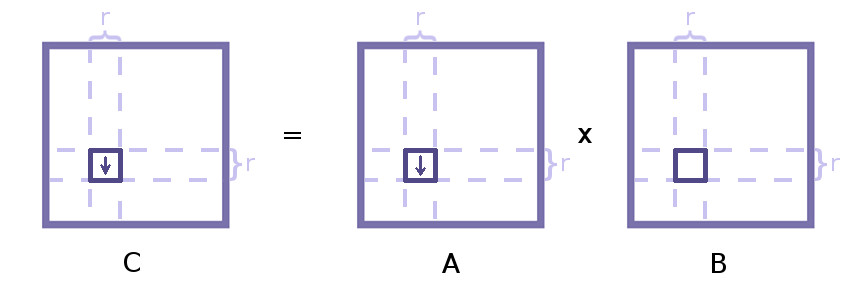
\includegraphics[width=0.60\textwidth]{IJKIJK_KKJJII.jpg}
    \caption{obszar danych wykorzystywanych w trzech wewnętrznych pętlach}
\end{figure}

Wykonując trzy pętle wewnętrzne, pojedynczy wątek przechodzi wielokrotnie każdy wiersz fragmentu macierzy A rozmiaru r x r, przechodzi wielokrotnie każdą kolumnę fragmentu maacierzy B rozmiaru r x r i jednokrotnie zapisuje każdy wiersz fragmentu macierzy C rozmiaru r x r.

\begin{figure}[H]
  \centering
    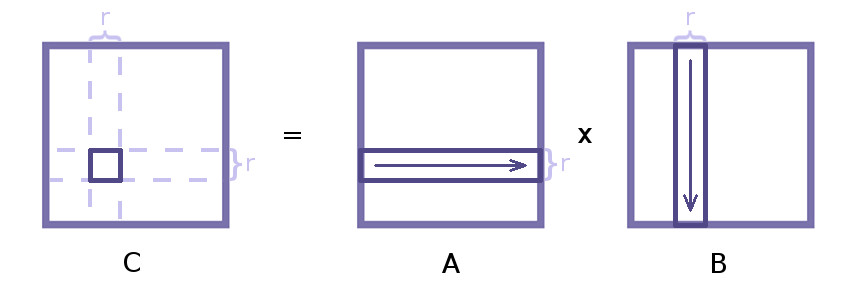
\includegraphics[width=0.60\textwidth]{IJKIJK_KKJJIIK.jpg}
    \caption{obszar danych wykorzystywanych w czterech wewnętrznych pętlach}
\end{figure}

Wykonując cztery pętle wewnętrzne, pojedynczy wątek wykorzystuje r wierszy macierzy A, r kolumn macierzy B oraz wypełnia fragment macierzy C o rozmiarze r x r.

\begin{figure}[H]
  \centering
    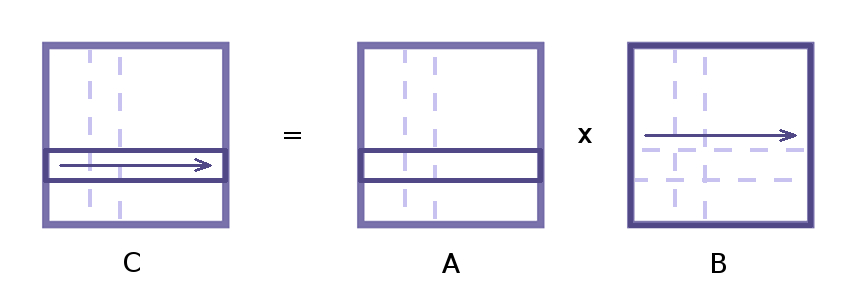
\includegraphics[width=0.60\textwidth]{IJKIJK_KKJJIIKJ.jpg}
    \caption{obszar danych wykorzystywanych we wszystkich wewnętrznych pętlach}
\end{figure}

Wykonując wszystkie pętle wewnętrzne, pojedynczy wątek wykorzystuje r wierszy macierzy A, całą macierz B oraz wypełnia r wierszy macierzy C.

\begin{figure}[H]
  \centering
    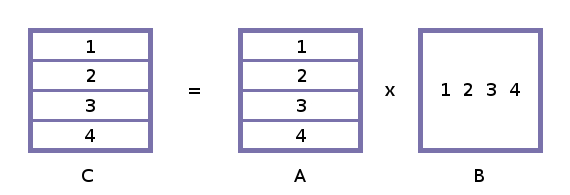
\includegraphics[width=0.60\textwidth]{IJK_KJI.jpg}
    \caption{podział pracy na wątki}
\end{figure}

Podział pracy na wątki jest taki sam jak w przypadku metody 3 pętlowej -  następuje przed najbardziej zewnętrzną pętlą, każdy wątek przechodzi osobne wiersze macierzy A i C, macierz B jest wykorzystywana w całości przez wszystkie wątki.


\subsection{False sharing}

Najmniejszą jednostką danych pobieranych do pamięci podręcznej jest linia pamięci (zwykle 64B). False sharing jest zjawiskiem występującym wtedy, gdy różne procesory wykonują operację zapisu różnych zmiennych znajdujących się w tej samej linii. Powoduje to unieważnienie kopii linii, znajdujących się w pamięciach podręcznych innych procesorów. Następnie dostęp do tych danych jest dla danego procesora wstrzymywany do momentu sprowadzenia aktualnej wersji linii pamięci. Mechanizm ten ma na celu zapewnienie spójności pamięci podręcznej. Częste występowanie takich sytuacji powoduje znaczący spadek efektywności przetwarzania.\\
\\
W analizowanych w zadaniu metodach podział pracy następuje przed pierwszą pętlą. Dzięki temu poszczególne procesory zapisują do rozłącznych, oddalonych od siebie obszarów pamięci. Jedynym miejscem, gdzie procesory mogłyby zapisywać dane do tej samej linii pamięci, są obszary w pobliżu granicy podziału macierzy wynikowej. Jest to niewielki procent danych, w porównaniu do rozmiaru całej wykorzystywanej macierzy. Ponadto, przetwarzanie na poszczególnych procesorach odbywa się w przybliżeniu w równym tempie, a więc nie wystąpi sytuacja, w której różne procesory będą naprzemiennie, wielokrotnie zapisywać do tej samej linii pamięci, ponieważ znajduje się ona na początku obszaru pracy jednego procesora i na końcu innego. Dane z macierzy źródłowych mogą być współdzielone przez procesory, nie stanowi to oczywiście problemu, ponieważ są to dane wyłącznie odczytywane. Można zatem stwierdzić, że problem false sharingu nie występuje w przypadku analizowanych algorytmów.

\subsection{Analiza lokalności czasowej}

Na prędkość przetwarzania, oprócz wydajności jednostek wykonujących operacje na danych (ALU, FPU), duży wpływ ma także czas dostępu do danych. Dostęp do danych, znajdujących się w pamięci operacyjnej, zajmuje stosunkowo dużo czasu, w porównaniu do tego, jak szybko procesor może wykonywać obliczenia. Spadek efektywności przetwarzania jest szczególnie zauważalny w przypadku, gdy kod cechuje się wysokim wskaźnikiem dostępu do danych. Rozwiązaniem problemu znacznych opóźnień do danych znajdujących się w RAM jest stosowanie w procesorach pamięci podręcznej, cechującej się znacznie lepszą przepustowością oraz mniejszymi opóźnieniami dostępu. Pamięć podręczna ma jednak bardzo ograniczoną pojemność, dlatego dla zapewnienia wysokiej efektywności przetwarzania ważne jest, aby kod charakteryzował czasową lokalnością odwołań do pamięci, tzn. aby dane raz sprowadzone do pamięci podręcznej były wielokrotnie wykorzystywane, zanim zostaną z niej usunięte.\\
\\
W trakcie analizy lokalności czasowej dostępu do danych metod wykorzystywanych w zadaniu przyjęto rozmiar pamięci podręcznej równy 6MB. Jest on równy pojemności współdzielonej pamięci L3. Pamięć L2 nie została wliczona, ponieważ niektóre dane mogą znajdować się zarówno w niej, jak i w pamięci trzeciego poziomu. Z kolei pojemność pamięci L1 jest tak mała, że nie miałaby znaczącego wpływu przy obliczaniu rozmiarów instancji. Ponadto należy pamiętać, że w systemie działają także inne procesy, w tym narzędzie do analizy wydajności AMD CodeXL, dlatego należy uwzględnić pewien zapas przy wyznaczaniu rozmiarów instancji.\\
\\
W przypadku metody 3 pętlowej (Listing \ref{lst:ijk}) w trakcie przetwarzania dane z macierzy B są wykorzystywane N razy. Konieczne jest zatem zmieszczenie całej macierzy B (o rozmiarze $n^2$) w pamięci podręcznej. Macierz ta może być współdzielona przez procesory.
Podział pracy przed pierwszą pętlą powoduje, że każdy procesor, w trakcie jednego przebiegu tej pętli, wielokrotnie wykorzystuje pojedynczy wiersz macierzy A, później nie odwołuje się ponownie do tych danych. Oznacza to, że w pamięci podręcznej muszą zmieścić się także 4 wiersze (każdy o rozmiarze $n$) macierzy A.
Konieczne jest również zmieszczenie 4 słów macierzy wynikowej (po jednym dla każdego procesora), jednak należy uwzględnić, że najmniejszą jednostką danych sprowadzanych do pamięci podręcznej jest linia (64B czyli 16 zmiennych typu float).\\
\\
Ostatecznie rozmiar instancji, dla której będzie zachowana lokalność czasowa dostępu do danych, można policzyć ze wzoru:
\begin{equation}
4 \cdot \left( n^2 + 4\cdot n + 4 \cdot 16 \right) < 6 \text{ MB}
\end{equation}

Uwzględniając pewien zapas daje to instancję o rozmiarze $n=1200$.\\
\\

W wersji 6 pętlowej algorytmu mnożenia macierzy (Listing \ref{lst:ijkiijjkk}) mamy do czynienia z podzieleniem całego zadania na etapy.Dzięki temu w danym czasie wielokrotnie korzystamy z mniejszej ilości danych (z każdej macierzy wykorzystujemy blok o wielkości $r \cdot r$ elementów). Umożliwia to zachowanie częściowej lokalności czasowej dostępu do danych (poszczególne bloki mogą być pobierane do pamięci podręcznej $n / r$ razy) dla większych instancji, dla których w przypadku poprzedniej metody konieczne byłoby pobieranie danych aż $n$ razy. Wartość $r$ musi być tak dobrana, aby iloraz $n/r$ był liczbą całkowitą. Ponieważ podział pracy następuje przed pierwszą pętlą, iloraz ten będzie również liczbą zadań do podziału między rdzeniami. Powinien być zatem liczbą podzielną przez 4 (liczba wykorzystywanych procesorów fizycznych) w celu zapewnienia zrównoważenia pracy systemu.\\
\\
Wielkość instancji zapewniającej częściową lokalność czasową można teoretycznie policzyć korzystając ze wzoru (TODO odnośnik do wzoru powyżej), zamiast $n$ podstawiając $r$. Wartość ta będzie poprawna przy założeniu, że rdzenie pracują z równą szybkością i w danych czasie mogą współdzielić ten sam wykorzystywany blok macierzy b. Jest to jednak założenie dość ryzykowne, więc do obliczenia przyjęto inny wzór: 
\begin{equation}
4 \cdot \left( 12r^2 \right) < 6 \text{ MB}
\end{equation}

Taki rozmiar powinien zapewnić, że dla każdego rdzenia możliwe jest przechowywanie w pamięci podręcznej wykorzystywanych przez niego aktualnie fragmentów (bloków r*r) wszystkich trzech macierzy. Daje to instancję testową o parametrach $n=1400$, $r=350$. Instancja ta zostanie również wykorzystana do testu metody 3 pętlowej, gdzie należy oczekiwać braku lokalności czasowej dostępu do danych, ponieważ wymagana pamięć podręczna musiałaby mieć pojemność ok. 7,5 MB.


\subsection{Analiza lokalności przestrzennej}

Współcześnie większość systemów korzysta z mechanizmu zarządzania pamięcią zwanego pamięcią wirtualną. Jedną z zalet takiej organizacji jest możliwość przydzielenia procesom działającym w systemie łącznie więcej pamięci niż rozmiar dostępnej fizycznej pamięci operacyjnej. Dane, które nie mieszczą się w pamięci operacyjnej i nie są aktualnie wykorzystywane są przechowywane w pliku wymiany na dysku twardym. Taka organizacja pamięci powoduje, że nie można już stosować adresów fizycznych, mających odwzorowanie bezpośrednio w pamięci RAM. Powszechnie stosowanym mechanizmem jest podział pamięci wirtualnej na strony (zwykle o rozmiarze 4 kB), stanowiące ciągły obszar pamięci. Pamięć RAM jest podzielona na ramki o rozmiarze odpowiadającym wielkości stron. Dana strona może aktualnie znajdować się w pamięci lub w pliku wymiany. Procesor posługuje się adresami logicznymi(wirtualnymi). W celu realizacji dostępu do danych, konieczna jest translacja adresu logicznego na aktualny adres fizyczny. Informacje umożliwiające określenie adresu ramki pamięci dla danej strony pamięci znajdują się w tablicy stron pamięci. Przeglądanie tablicy stron przy każdym dostępie do pamięci byłoby bardzo kosztowne i znacząco zmniejszałoby efektywność przetwarzania. Dlatego tutaj również stosuje się pewien rodzaj pamięci podręcznej - bufor translacji adresu (TLB). Posiada on stałą liczbę par adresów stron i odpowiadających im ramek i pozwala na szybkie odwzorowanie (zwykle w jednym cyklu zegarowym) adresu wirtualnego na adres fizyczny.\\
\\
Procesor wykorzystywany w zadaniu posiada bufor TLB o pojemności 544 par adresów (na każdy rdzeń). Strona pamięci wirtualnej ma rozmiar 4 kB (czyli mieści 1024 zmienne typu float).\\
\\
W celu zapewnianie efektywnego dostępu do adresów w buforze translacji w wersji 3 pętlowa algorytmu mnożenia macierzy musi on zmieścić:
\begin{itemize}
\item adresy wszystkich stron zawierających macierz B,
\item adresy stron zawierających jeden wiersz macierzy A,
\item adres strony zawierającej jedną komórkę macierzy C
\end{itemize}

Rozmiar instancji można wyznaczyć posługując się wzorem (uwzględniono możliwość, że macierze nie będą wyrównane do początku strony, dlatego do pierwszego i drugiego wyrazu dodano 1):
\begin{equation}
\ceil*{\frac{n^2}{1024}} + 1 + \ceil*{\frac{n}{1024}} + 1 + 1 < 544
\end{equation}

Dodatkowo przyjmując pewien zapas dla innych procesów działających w systemie, daje to instancję o rozmiarze $n=700$, w przypadku której dane mogą być rozmieszczone na maksymalnie 483 stronach.\\
\\
W przypadku wersji 6 pętlowej określenie odpowiednich wartości n oraz r jest trudniejsze. Jeden blok o wielkości r*r może znajdować się na r stronach (np. przy n=1024, r=256 i odpowiednim wyrównaniu danych). W przypadku braku wyrównania, może to być już 2r stron lub więcej dla bardzo dużych instancji.\\
\\
Eksperyment zostanie zatem przeprowadzony dla instancji:
\begin{enumerate}
\item n=1400, r=350
\item n=1400, r=175
\end{enumerate}

Obie instancje zapewniają równomierne rozłożenie pracy na wątki. Pierwsza instancja nie zapewni lokalnego przestrzennie dostępu do danych, ponieważ rozmiar macierzy będzie powodował takie ułożenie danych na stronach, że przynajmniej niektóre bloki będą wymagały 2r stron (czyli 700), co przy wielokrotnym wykorzystywaniu fragmentu macierzy B będzie skutkowało wielokrotnym zastępowaniem wpisów w TLB i koniecznością ponownego uzupełniania tych informacji. Druga instancja nawet przy pesymistycznym założeniu dotyczącym rozmieszczenia danych na stronach zapewni lokalność przestrzenną (adresy 350 stron dla fragmentu macierzy B oraz pojedynczych stron dla fragmentów macierzy A oraz C zmieszczą się w buforze).\\
\\
Dodatkowo sprawdzona zostanie efektywność przetwarzania dla instancji:
\begin{enumerate}
\item n=2800, r=350
\item n=2800, r=700
\end{enumerate}

Pierwsza może charakteryzować się zbliżoną lokalnością czasową do instancji $n=1400$, $r=350$, choć w tym przypadku dane mogą być pobierane ośmiokrotnie ($n/r = 8$). W przypadku drugiej instancji lokalność czasowa wciąż może być zachowana. Chociaż nie jest spełniony warunek ze wzoru (TODO odnośnik), to przy optymistycznym założeniu, że rdzenie pracują z podobną prędkością, fragment macierzy B może być współdzielony, z macierzy A wystarczy teoretycznie zmieścić w pamięci podręcznej jeden wierz bloku r*r, a z macierzy wynikowej jedną linię zawierającą aktualnie obliczaną komórkę macierzy. Z drugiej strony, należy spodziewać się znaczącego wzrostu wskaźnika braków trafień do TLB, ponieważ, niezależnie od sposobu ułożenia danych na stronach, adresy stron zawierających fragment r*r macierzy B nie zmieszczą się w buforze TLB, co będzie powodować konieczność przeglądania tablicy stron przy każdym dostępie do danych tej macierzy, wewnątrz najbardziej wewnętrznej pętli.

\section{Eksperyment pomiarowy}

\subsection{Instancje}

\begin{table}[H]
\centering
\def\arraystretch{1.5}
\begin{tabular}{|c|}
\hline
metoda 3 pętlowa \\
\hline
n \\
\hline
700 \\
\hline
1200 \\
\hline
1400 \\
\hline
\end{tabular}
\hspace{70pt}
\begin{tabular}{|c|c|}  %druga tabela
\hline
\multicolumn{2}{|c|}{metoda 6 pętlowa} \\
\hline
n & r\\
\hline
1400 & 350 \\
\hline
1400 & 175 \\
\hline
2800 & 700 \\
\hline
2800 & 350 \\
\hline
\end{tabular}
\end{table}

\subsection{Mierzone parametry}

W trakcie eksperymentu zmierzono czas przetwarzania danej instancji odpowiednią metodą oraz czas przetwarzania tej samej instancji sekwencyjną metodą IKJ, w celu wyznaczenia wartości parametru przyspieszenia przetwarzania równoległego.\\
\\
W celu obliczenia przedstawionych dalej miar efektywności dokonano pomiaru następujących zdarzeń w narzędziu do analizy wydajności AMD CodeXL:

\begin{itemize}
\item \textbf{CPU clocks not halted},
\item \textbf{Retired instructions},
\item \textbf{Data cache accesses},
\item \textbf{L1 DTLB and L2 DTLB miss},
\item \textbf{L3 miss}.
\end{itemize}

Każdy kod został uruchomiony dwukrotnie, ponieważ jednocześnie, z odpowiednią dokładnością, można mierzyć tylko 4 zdarzenia. Progi zliczania zostały zapisane w załączonym pliku, zwykle były to wartości domyślne, jednak w niektórych przypadkach, przy bardzo małej wartości wartości progów zostały zmniejszone.

\subsection{Wyniki eksperymentu}

todo, odwołanie do tabeli, podpisać je w arkuszu i tu używać tych oznaczeń

\subsection{Wzory}

{\huge TODO przedziały wartości}

Prędkość przetwarzania
\begin{equation}
\frac{Z}{Tobl} = \frac{2 \cdot n^3}{Tobl}
\end{equation}

Liczba instrukcji na cykl procesora IPC1 dla procesora
\begin{equation}
\frac{LIA}{LCP}
\end{equation}

Liczba instrukcji na cykl procesora IPCS dla systemu
\begin{equation}
\frac{LPF \cdot LIA}{LCP}
\end{equation}

Wskaźnik braków trafień
\begin{equation}
\frac{BTL3}{LIA}
\end{equation}

Wskaźnik dostępu
\begin{equation}
\frac{LDP}{LIA}
\end{equation}

Wskaźnik braków trafień do głównego bufora translacji adresów danych
\begin{equation}
\frac{BTBT}{LIA}
\end{equation}

Krotność pobierania danych instancji do pamięci podręcznej
\begin{equation}
\frac{BTL3 \cdot dlpp}{wtz \cdot 3 \cdot n \cdot n}
\end{equation}

Miara kosztu synchronizacji
\begin{equation}
\frac{CCP - CWP}{CCP} = \frac{LUPF \cdot Tobl - LCP \cdot Tclk}{LUPF \cdot Tobl}
\end{equation}

Przyspieszenie przetwarzania równoległego  %TODO - co z polskimi literami?
\begin{equation}
Sp(równoległe\; A) = \frac{Tobl(obliczenia\; sekwencyjne\; IKJ)}{Tobl(obliczenia\; równoległe\; A)}
\end{equation}


\subsection{Obliczenia}
todo: BINDy np. LIA - Ret inst

przygotować szblony wykresów, na razie nie  wiem dla których dokładnie danych 


%\begin{figure}[H]
%  \centering
%    \includegraphics[width=0.60\textwidth]{img}
%    \caption{jklfjgskl fdsfsd}
%\end{figure}







\section{Wnioski}
{\huge TODO uwaga zmiana wzoru na wskaźniki TLB-miss-rate}\\

\subsection{Metoda 3 pętlowa}

Wielkości instancji charakterystycznych obliczone w czasie analizy warunków lokalności czasowej i przestrzennej dostępu do danych, zgodnie z oczekiwaniami cechują się różną prędkością przetwarzania. Największą wartość uzyskano dla instancji $n=700$, która cechuje się dwoma rodzajami lokalności  dostępu do danych. W przypadku instancji $n=1200$, dla której miała być zachowana tylko lokalność czasowa, prędkość przetwarzania jest zauważalnie niższa. Instancja $n=1400$ cechuje sie brakiem lokalności dostępu do danych, co skutkuje zdecydowanie wolniejszym przetwarzaniem.\\
\\
Pomiar wymienionych wcześniej zdarzeń pozwolił na wyznaczenie m. in. wskaźników braków trafień do pamięci podręcznej oraz do bufora translacji. Wskaźnik braków trafień do TLB jest o rząd wielkości mniejszy w przypadku instancji zapewniającej lokalność przestrzenną. Na liczbę trafień od bufora mają również wpływ inne działające procesy, jednak w przypadku instancji $n=700$ przewidziany został pewien zapas. Nie bez znaczenia jest również fakt, że macierze były najpierw inicjowane liczbami losowymi (macierze A i B), oraz zerami (macierz wynikowa). W związku z tym wiele adresów mogło być już obecnych w buforze, a zatem uzupełnianie nie było wcale wymagane. Bardzo niska wartość wskaźnika ma więc sens, można stwierdzić, że adresy stron wykorzystywanych wielokrotnie były prawie zawsze dostępne w buforze. W obu instancjach nie zapewniających lokalności przestrzennej wskaźnik braków trafień miał podobną, wyższą wartość, spowodowaną koniecznością uzupełniania adresów stron zawierających dane z macierzy B.\\
\\
Analizując wskaźnik braków trafień do pamięci podręcznej, oraz wartość określającą ile razy dane instancji były pobierane (TODO odnośnik do tabeli) można zauważyć, że dla instancji mającej zapewniać lokalność czasową - $n=1200$ a nawet dla mniejszej instancji $n=700$, dane były pobierane z pamięci operacyjnej więcej niż raz. Jest to prawdopodobnie spowodowane działaniem w systemie innych procesów, co powodowało usuwanie z pamięci podręcznej niektórych rzadziej używanych w czasie obliczeń danych. Z kolei w przypadku instancji $n=1400$ łatwo dostrzec brak lokalności czasowej. Wskaźnik braków trafień jest o rząd wielkości wyższy niż w przypadku $n=1200$ a dane instancji były pobierane ponad 904 razy. Wzór odnosi się jednak do wielkości wszystkich macierzy, a sposób przeglądania macierzy A oraz B zapewnia lokalność dostępu, dlatego też można stwierdzić, że dane macierzy B były wielokrotnie zastępowane i ponownie sprowadzane do pamięci podręcznej.\\
\\
Wartość przyspieszenia przetwarzania równoległego jest z kolei najwyższa dla instancji bez lokalności czasowej oraz przestrzennej ($n=1400$). Jest to jednak spowodowane tym, że metoda sekwencyjna IKJ, służąca jako odniesienie, charakteryzowała się znacząco niższą efektywnością przetwarzania dla tej instancji. Jest to spowodowane również częściowym brakiem lokalności dostępu do danych metody IKJ w przypadku tej instancji, co pokazują wyniki dodatkowego pomiaru zdarzeń w CodeXL dla metody sekwencyjnej (TODO odnośnik tabela).\\
\\
Miara IPC, określająca średnią liczbę instrukcji wykonywanych w cyklu zegarowym procesora, zgodnie z oczekiwaniami wskazuje na trend zgodny z prędkością przetwarzania.


\subsection{Metoda 6 pętlowa}

Wielkości wskaźników dotyczących lokalności czasowej dostępu do danych (TODO odnośnik do tabeli) pokazują, że wielkość macierzy nie większego znaczenia, ważny jest natomiast rozmiar bloku przetwarzanego w danym etapie. W przypadku instancji $n=1400$ nieco korzystniejsze dla efektywności przetwarzania wartości zaobserwowano dla instancji $r=350$. Nie jest to zaskakujący rezultat, ponieważ instancja $r=175$, mimo że może być mniej wrażliwa na czynniki zewnętrzne (zajmowanie części zasobów przez inne procesy) ponieważ posiada większy zapas, to podział pracy na 8 etapów powoduje, że dane bloki danych wykorzystywane ponownie w kolejnych etapach są sprowadzane 2 razy więcej razy. W przypadku instancji $n=2800$, $r=350$ wartość wskaźnika braków trafień do pamięci podręcznej zgodnie z oczekiwaniami jest zbliżoną do tej, która została uzyskana dla instancji $n=1400, r=350$. Zwiększyła się krotność pobierania danych instancji do pamięci podręcznej, ponieważ liczba etapów  przetwarzania wynosi 8. W przypadku instancji $n=2800, r=700$ lokalność czasowa dostępu do danych w trakcie poszczególnych etapów przetwarzania również została zachowana.\\
\\
Znaczące różnice zaobserwowano natomiast w kwestii lokalności przestrzennej dostępu do danych. Zgodnie z oczekiwaniami, najlepszy wynik otrzymano dla instancji $n=1400, r=175$. Przy $r=350$ wskaźnik braków trafień do TLB miał wartość większą o jeden rząd wielkości. Pełna lokalność przestrzenna nie została zachowana, jednak wartość wskaźnika rzędu $10^{-3}$ nie powoduje jeszcze znaczącego spadku prędkości przetwarzania. Dla instancji $n=2800$ wskaźnik ten ma wartość ok. 2 razy większą niż dla $n=1400$. Jest to ponownie spowodowane podziałem pracy na 8 etapów (a nie 4), więc liczba koniecznych uzupełnień brakujących adresów wzrasta proporcjonalnie.
Ostatnia instancja $n=2800, r=700$ charakteryzuje się, zgodnie z przewidywaniami, całkowitym brakiem lokalności przestrzennej. Wartość wskaźnika braków trafień do TLB wynosi około 25\%, co oznacza, że bufor translacji zawierał jedynie pary adresów potrzebne przy odczycie oraz modyfikacji aktualnie wykorzystywanych wartości w macierzy wynikowej, oraz przy odczycie danych z macierzy A. Przy próbie dostępu do danych z fragmentu macierzy B (zawsze kolejne komórki w ramach kolumny), zawsze następował brak trafienia do bufora translacji adresów.\\
\\
Powyższe fakty mają odzwierciedlenie w prędkości przetwarzania. Najgorszą wartość uzyskano dla instancji $n=2800, r=700$, natomiast pozostałe instancje cechowały się zbliżoną prędkością przetwarzania. Wartość wskaźnika IPC ponownie znajduje odzwierciedlenie w prędkości przetwarzania. W przypadku instancji analizowanych w tym punkcie algorytm sekwencyjny IKJ cechował się niemal stałą prędkością przetwarzania, a zatem można zaobserwować zgodne z oczekiwaniami przyspieszenie przetwarzania równoległego dla instancji cechujących się przynajmniej częściową lokalnością. W przypadku instancji $n=2800, r=700$ przetwarzanie równoległe odbywało się ponad 2 razy wolniej, niż w metodzie sekwencyjnej IKJ.\\
\\
Na podstawie analizy wyników obu metod można zatem wyciągnąć wniosek, że problem z lokalnym czasowo dostępem do danych powoduje spadek efektywności przetwarzania, jednak znacznie większe znaczenie ma brak lokalności przestrzennej.

\end{document}